% !TeX spellcheck = en_US
% !TeX root = ../Tom_Sandmann-master_thesis
\section{Architecture}
In this section, we describe the architecture of the hardware design of {\fourq} as proposed in \cite{jarvinen2016four}.

\subsection{Core}
An overview of the architecture of the field arithmetic unit (FAU) (also referred to as ``the core'') can be seen in \Cref{fig: fourQ hardware architectural diagram}.
%
\begin{figure}
	\centering
	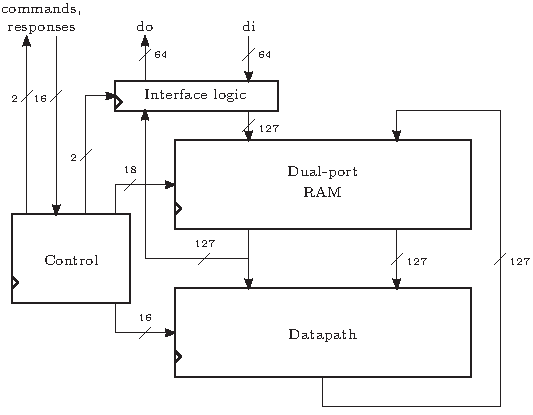
\includegraphics[scale=1.0]{fourq_hardware_architecture_diagram}
	
	\captionof{figure}{Architectural diagram of the core {\fourqs} hardware design proposed in \cite{jarvinen2016four}.}
	\label{fig: fourQ hardware architectural diagram}
\end{figure}
%
The interface logic is used to give inputs to the architecture and to retrieve outputs.
Values used in the computation of the scalar multiplication are stored in the Dual-Port RAM.
The Dual-Port RAM is implemented as BlockRAM in the FPGA. 
By default, the host is connected to the architecture through a 64-bit interface.
Using this interface, we can write or read a value at a specific address within this RAM.
As the design only uses 128-bit data values, this address indicates whether the higher or lower part of the 128-bit word is being written or read.
Although the width of the interface is 64-bits by default, this width can easily be changed \cite{jarvinen2016four}.
The datapath within the design is responsible for the field operations.
It provides the basic operations needed to allow the implementation of field addition, subtraction, doubling and multiplication.
It performs these operations in $\mathbb{F}_{p^2}$ (which in case of {\fourq} boils down to complex number arithmetic).
The datapath consists of two paths: a multiplier path and an adder/subtractor path \cite{jarvinen2016four}.
%
\begin{itemize}
	\item The \textbf{multiplier path} is build around a pipelined 64x64 bit multiplier build using DSP blocks.
	The pipelined multiplier consists of seven pipeline stages (as can be seen in \Cref{sec: IP Blocks}), and the multiplication is done using the schoolbook algorithm.
	To compute the result of a multiplication, four $64 \times 64$-bit partial multiplications are done: $a_i \times b_j$ for $i, j \in \{0, 1\}$.
	This gives $a = a_1 2^{64} + a_0$ and $b = b_1 2^{64} + b_0$.
	The results of these partial multiplications are accumulated in a 256-bit register.
	The order in which the partial products are stored is as follows: $(i, j) = (0, 0), (0, 1), (1, 0), (1, 1)$.
	After $(0, 0)$ and $(1, 0)$, the register is shifted down by 64 bits.
	
	\item The \textbf{adder/subtractor} is responsible for computing the additions, subtractions and modular reductions of the partial multiplications results.
	The adder/subtractor path is designed in such a way that it can also be used when the multiplier path is performing a multiplication \cite{jarvinen2016four}. 
	This is only possible if the modular reduction computed is available and by introducing an additional set of input registers to the adder/subtractor.
	The adder/subtractor also allows accumulation of its results in the output register. 
	Therefore, most of the additions and subtractions required during scalar multiplication come for free.
\end{itemize}
%

\subsection{Control logic} \label{subsec: Control Logic}
The control unit is responsible for controlling the datapath and the memory, and therefore implements all the levels required by {\fourqs} scalar multiplication.
The control logic consists of a program ROM that consists of instruction lines for the datapath and memory addresses.
In addition, the control logic contains a FSM that controls the read addresses from the program ROM.
Also a decoder is present to decode the instructions in the program ROM to control signals such that they can be used to control the datapath and the memory components.
The program ROM contains 8015 lines of hand-optimized instructions.
These instructions are 25 bits wide:
3 bits are used for the multiplier path, 5 bits for the adder/subtractor path, one bit for write enable and two 8-bit memory addresses for the RAM \cite{jarvinen2016four}.
Each instruction line is executed in one clock cycle.
The program ROM is divided into \emph{seven} different routines.
Given a base point $P = (x, y)$ and following \cite[Algorithm 1]{jarvinen2016four}, the routines are as follows:
%
\begin{itemize}
	\item \emph{Initialization}: Lines 1-14 map the affine point $P$ to the representation $\bm{R_1}$: $X \gets x, Y \gets y, Z \gets 1, T_a \gets x$ and $T_b \gets y$.

	\item \emph{Precomputation}: Lines 15-4199 calculate the lookup table $T$ by making use 
	of the endomorphisms and point additions. $T$ consists of 8 points in total, each represented in $\bm{R_5}$.
	
	\item \emph{Initialization main loop}: Lines 4200-4214 initialize the point accumulator (which is used in the main loop) by loading a point from the lookup table $T$. This is done by making use of the first digit of the recoded multiscalar and by mapping this point to representation $\bm{R_4}$. 
	
	\item \emph{Main loop}: Lines 4215-4568 compute the point doubling $Q \gets [2]Q$ and addition $Q \gets Q + m_i \cdot T[v_i]$. The point doubling is calculated using representation $\bm{R_1 \gets R_4}$ (i.e. the input representation to this operation is $\bm{R_4}$, and the output representation is $\bm{R_1}$), while the point addition is calculated using representation $\bm{R_1 \gets R_1 \times R_2}$.
	
	\item \emph{Affine conversion}: Lines 4569-7437 map the resulting point, represented in $\bm{R_1}$, to affine coordinates by computing $x = X/Z$ and $y = Y/Z$. The majority of these lines are used to perform an inversion in $\mathbb{F}_p$.
	
	\item \emph{Point validation}: Lines 7438-7561 verify whether the base point $P=(x, y)$ is in $\mathcal{E}(\mathbb{F}_{p^2})$. This boils down to verify whether point $P$ satisfies the curve equation $-x^2 + y^2 - 1 -dx^2y^2 = 0$.
	
	\item \emph{Cofactor clearing}: To prevent small subgroup attacks (which can be performed in specific scenarios) \cite{lim1997key}, we can perform cofactor clearing as described in \cite[Appendix A]{costello2015fourq}. Lines 7562-8014 perform the cofactor killing by computing $392P$. This is done by making use of the $\bm{R_2 \gets R_1}$ map (lines 7562-7643), followed by eight point doublings (lines 7644-7799) and two point additions (lines 7800-7643).
\end{itemize}
%
As mentioned previously, the instruction decoder controls how the instructions, read from the program ROM, are decoded to appropriate control signals.
The FSM of the control is responsible for setting the address for the program ROM. 
This is done by making use of a counter and hard-coded pointers to the beginning of each routine within the program ROM.
Depending on the operation, the counter gets either incremented such that the next line of a routine is fetched, or its value is set to the appropriate routine.
Once the end pointer of a routine is reached, either the pointer moves to the start of another routine, or the FSM moves to the wait state.

\subsection{Scalar decompose \& recode unit}
The decompose unit of the scalar unit is responsible for both decomposing the scalar $m$ into the 64-bit multiscalars $a_1, a_2, a_3, a_4$ (as described in \Cref{subsec: Scalar decomposition}), and to recode these scalars into digit-columns $(d_{64}, \ldots , d_0)$ with $0 \le d_i < 16$.
These digit-columns are then used during the scalar multiplication to retrieve the correct precomputed points to be added.
To calculate the multiscalar, the four curve constants $\ell_1, \ell_2, \ell_3, \ell_4$ and the values of the basis $\bm{b} = (\bm{b_1}, \bm{b_2}, \bm{b_3}, \bm{b_4})$ are necessary.
As these values are all constants, they are stored in the program ROM and are used from there on.
In addition, the values $\hat{\alpha}_i$ for $i \in \{1, \ldots, 4 \}$ need to be computed, which is done by computing $\ell_i m / \mu$ with $\mu := 2^{256}$.
As the computation of these value involves a multiplication, a \emph{truncated multiplier} was designed in \cite[Algorithm 3]{jarvinen2016four}.
Given two integers $X$ and $Y$ with $0 \le X < 2^{256}$ and $0 \le Y < 2^{195}$, the result $Z_H = \left \lfloor X \cdot Y / (2^{256})\right \rfloor \pmod{2^{64}}$ is calculated.
The truncated multiplier can also be used to calculate the result $Z_L = XY \pmod{2^{64}}$, which is necessary to compute the final values of $a_i$.
Most of the functionality of the truncated multiplier is due to the $17 \times 264$-bit \emph{row multiplier}.
The row multiplier computes the product $Y_j \cdot X$ for a $j \in [0, 11]$ (as needed in \cite[Algorithm 3 line 5]{jarvinen2016four}.) 
The row multiplier is implemented by making use of DSP blocks (11 in total).
The Xillinx Zynq FPGA family, that was used to test the proposed hardware design of {\fourq}, provides $17\times 24$ unsigned integer multiplication with an addition of a 47-bit unsigned integer. 
To be compliant with these dimensions, the 256-bit input integer $X$ is split into $\lceil 256 / 24 \rceil = 11$ blocks of 24-bit words, and the 195-bit input integer $Y$ is split into $\lceil 195 / 17 \rceil = 12$ blocks of 17-bit words.
$X$ and $Y$ now become represented as $X_{10}, X_9, \ldots, X_0$ and $Y_{11}, X_{10}, \ldots Y_0$ in radix $2^{24}$ and $2^{17}$ respectively.

The recode unit is also implemented as FSM, where each state computes one or more lines of the recoding algorithm presented in \cite{costello2015fourq}.
